\documentclass[12pt, a4paper]{article}

\usepackage{enumerate}
\usepackage{multicol}
\usepackage{listings}
\usepackage{graphicx}

\lstset{
	breaklines=true
}

\setlength\parskip{1em}
\setlength\parindent{0em}

\title{Assignment 1}

\author{Hendrik Werner s4549775}

\begin{document}
\maketitle

\section{} %1
\begin{enumerate}[a]
	\item %a
	\begin{multicols}{2}
		I found 2 network interfaces. One is the localhost (lo) and one is an ethernet interface (eth0).

		\begin{tabular}{c|c}
			Network Interface & IP4\\\hline
			eth0 & 10.0.2.15\\
			lo & 127.0.0.1\\
		\end{tabular}
	\end{multicols}

	\item %b
	\paragraph{ping}
	I began by capturing the traffic on eth0 and issued the command "ping ru.nl". I stopped the process after 4 pings.

	This resulted in a broad casted ARP request to ask who has IP 10.0.2.3. After this request was answered a DNS lookup for ru.nl was issued and the answer contained ru.nl's IP4 address to which a ICMP ping was sent and an answer received. This step was repeated until the process was stopped.

	Interleaved with that was another ARP request to ask who 10.0.2.2 was but I don't know why. This address wasn't used after that.

	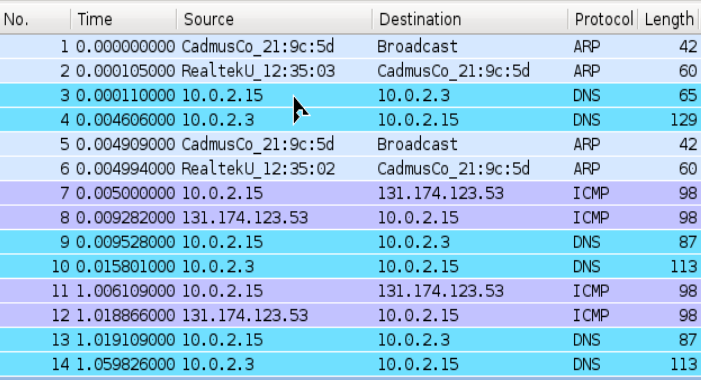
\includegraphics[width=\linewidth]{images/ping}

	I expected the DNS requests to be cached but they were not. For each new ping there was another DNS lookup. The rest is pretty obvious: A request is sent to the looked up IP and an answer received. Then this is repeated until the user stops the process.

	\paragraph{traceroute}
	Next I used "traceroute google.com". The first thing it did was request the A and AAAA records for google.com over DNS. It received the IPv4, and IPv6 addresses of Google. I don't know why the IPv6 address was requested. It was not used. Maybe it would have been used if google.com had not had an IPv4 address.

	Next traceroute began sending UDP packets with increasing TTL (time to live). Those requests exceeded theit TTL somewhere along the way to google.com and the corresponding node sent an error in the ICMP protocol back to traceroute. This allows it to be identified as a hop on the route.

	By repeatedly doing this Wireshark can identify the whole route to google.com.

	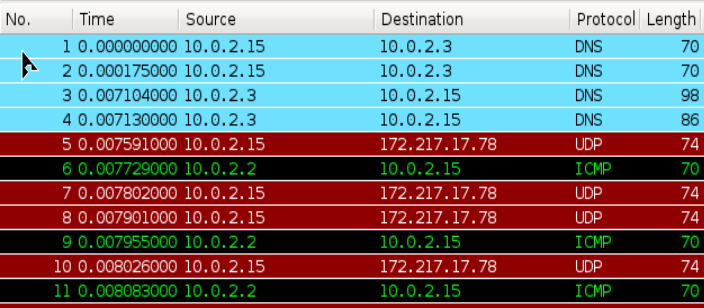
\includegraphics[width=\linewidth]{images/traceroute}

	\paragraph{whois}
	As advised I ran "whois 128.119.245.12". Just like traceroute it began by requesting the A and AAAA records of whois.arin.net but proceeded to ignore the IPv6 address.

	It then sent a lot of TCP packets to this address and got a lot of responses. I was told that some of those TCP packets were actually the WHOIS protocol but NetKit did not identify it as such. It contained Wireshark 1.8.2 which is quite old.

	I found the first request that contained the requested IP (128.119.245.12) and clicked "follow TCP Stream".

	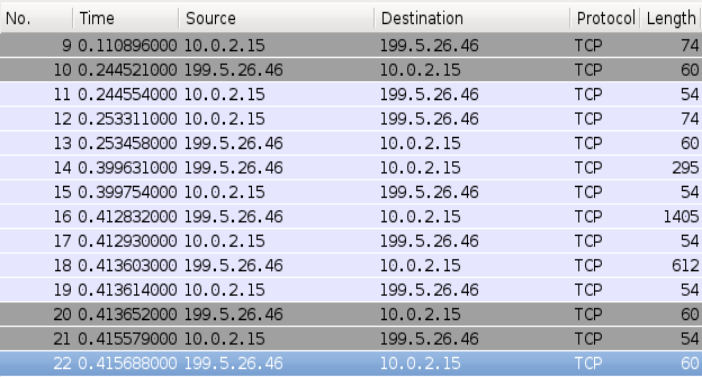
\includegraphics[width=\linewidth]{images/whois}

	If you create a website you have to register it to someone. You have to provide the information you can retrieve with whois. Whois just requests the information from the database and displays it.
\end{enumerate}

\section{} %2
\begin{enumerate}[a]
	\item %a
	I used the filter "http and ip.src == 128.119.245.12" to filter out only HTTP request that originated from the server.

	\item %b
	HTTP stream:

	\begin{lstlisting}
GET /wireshark-labs/INTRO-wireshark-file1.html HTTP/1.1
Host: gaia.cs.umass.edu
Connection: keep-alive
Upgrade-Insecure-Requests: 1
User-Agent: Mozilla/5.0 (X11; Linux x86_64) AppleWebKit/537.36 (KHTML, like Gecko) Chrome/56.0.2924.76 Safari/537.36
Accept: text/html,application/xhtml+xml,application/xml;q=0.9,image/webp,*/*;q=0.8
Accept-Encoding: gzip, deflate, sdch
Accept-Language: en-US,en;q=0.8,de;q=0.6

HTTP/1.1 200 OK
Date: Thu, 02 Feb 2017 13:23:01 GMT
Server: Apache/2.4.6 (CentOS) OpenSSL/1.0.1e-fips PHP/5.4.16 mod_perl/2.0.10 Perl/v5.16.3
Last-Modified: Thu, 02 Feb 2017 06:59:01 GMT
ETag: "51-54786b33397f0"
Accept-Ranges: bytes
Content-Length: 81
Keep-Alive: timeout=5, max=100
Connection: Keep-Alive
Content-Type: text/html; charset=UTF-8

<html>
Congratulations!  You've downloaded the first Wireshark lab file!
</html>
	\end{lstlisting}
\end{enumerate}

\section{} %3
\begin{enumerate}[a]
	\item %a
	Output of "traceroute soest.hawaii.org":

	\begin{lstlisting}
traceroute to soest.hawaii.edu (128.171.151.230), 30 hops max, 60 byte packets
 1  mijnmodem.kpn.home (192.168.2.254)  0.801 ms  0.792 ms  0.875 ms
 2  195.190.228.52 (195.190.228.52)  2.172 ms  2.167 ms  2.162 ms
 3  nl-ah-dc2-git-cr01.kpn.net (213.75.1.77)  6.605 ms nl-rt-dc2-git-cr04.kpn.net (213.75.64.241)  5.881 ms 77.1.75.213.in-addr.arpa (213.75.1.77)  6.594 ms
 4  nl-rt-dc2-ice-ir01.kpn.net (213.75.64.240)  6.588 ms nl-asd-dc2-ice-ir01.kpn.net (213.75.1.76)  6.572 ms 240.64.75.213.in-addr.arpa (213.75.64.240)  6.574 ms
 5  rt2-rou-1022.NL.eurorings.net (134.222.93.140)  5.844 ms asd2-rou-1022.NL.eurorings.net (134.222.93.138)  5.093 ms  5.091 ms
 6  chg-s1-rou-1041.US.eurorings.net (134.222.48.90)  100.393 ms  98.856 ms  98.855 ms
 7  nyk-s2-rou-1021.US.eurorings.net (134.222.48.35)  87.234 ms  87.232 ms  87.222 ms
 8  xe-4-0-3.0.rtsw.seat.net.internet2.edu (64.57.20.168)  141.577 ms  141.062 ms  141.055 ms
 9  ae-0.0.rtr.eqch.net.internet2.edu (64.57.20.33)  109.729 ms 64.57.21.50 (64.57.21.50)  205.772 ms  205.778 ms
10  xe-4-0-3.0.rtsw.seat.net.internet2.edu (64.57.20.168)  151.076 ms  151.072 ms xe-1-1-0-53-coconut-re0.uhnet.net (205.166.205.27)  205.760 ms
11  64.57.21.50 (64.57.21.50)  216.341 ms  215.357 ms  215.339 ms
12  vl-3208-manoa6506-1.uhnet.net (128.171.186.163)  206.740 ms  206.396 ms xe-1-1-0-53-coconut-re0a.uhnet.net (205.166.205.27)  215.318 ms
13  128.171.186.241 (128.171.186.241)  207.136 ms  207.384 ms  208.155 ms
14  163.186.171.128.in-addr.arpa (128.171.186.163)  216.442 ms soestgw.soest.hawaii.edu (128.171.124.9)  208.804 ms  209.786 ms
15  tenghig.soest.hawaii.edu (128.171.150.3)  207.301 ms 128.171.186.241 (128.171.186.241)  217.043 ms 3.150.171.128.in-addr.arpa (128.171.150.3)  208.048 ms
16  dns.soest.hawaii.edu (128.171.151.230)  207.226 ms  207.224 ms  206.921 ms
	\end{lstlisting}

	\item %b
	The number of hops (that I can see) on the way to the server is 16.

	I used "ping soest.hawaii.edu" and let it run for 10 pings. The variance was \textbf{very} low at $0.5ms$ and the average rountrip time was 206ms.

	\item %c
	\begin{multicols}{2}
		I obtained the following table using $whois$.

		\begin{tabular}{l|c}
		\multicolumn{1}{c|}{IPv4} & Location\\\hline
		192.168.2.254 & Local router (Netherlands)\\
		195.190.228.52 & Netherlands\\
		213.75.* & Netherlands\\
		134.222.93.* & Netherlands\\
		134.222.48.* & Mainland USA\\
		64.57.* & Mainland USA\\
		205.166.205.27 & Hawaii (USA)\\
		128.171.* & Hawaii (USA)
		\end{tabular}

		Oceans are crossed between Hop 5 and Hop 6, as well as Hop 10 and Hop 11. This is consistent with big jump in the RTT.
	\end{multicols}
\end{enumerate}

\section{} %4
\begin{enumerate}[a]
	\item %a
	\item %b
	\item %c
\end{enumerate}

\section{} %5
\begin{enumerate}[a]
	\item %a
	\item %b
	\item %c
\end{enumerate}

\end{document}
